\documentclass[10pt]{report}            % Report class in 11 points
\usepackage{mathtools}
\usepackage{amssymb,amsmath}
\usepackage{graphicx}
%\oddsidemargin 5pt
\parindent0pt  \parskip10pt             % make block paragraphs
\raggedright                            % do not right-justify
\title{\bf CSCI576 Assignment 2 Report}  % Supply information

\author{Hengyue Liu\\USC ID: 4107-2966-75}              %   for the title page.
\date{\today}                           %   Use current date.

\begin{document}                        % End of preamble, start of text.
\maketitle                              % Print title page.
\pagenumbering{roman}                   % roman page number for toc
\setcounter{page}{2}                    % make it start with "ii"
%\tableofcontents                        % Print table of contents
\renewcommand{\chaptername}{Part}
%\renewcommand{\thechapter}{\Alph{chapter}}
\chapter{Written Questions}                % Print a "chapter" heading
\pagenumbering{arabic}                  % Start text with arabic 1

 
\section*{Q 1}                  % Print a "section" heading
\par Proof:

The chromaticity coordinates $(x_c,y_c)$ are computed by the projective transformation:
$x_c=\frac{X}{X+Y+Z}, y_c=\frac{Y}{X+Y+Z}$,\\
then $\frac{1-x_c-y_c}{y_c}\cdot Y=\frac{Z}{(X+Y+Z)\cdot y_c}\cdot Y=\frac{Z}{Y}\cdot Y=Z$.                      
  

 \section*{Q 2}                  % Print a "section" heading
 Solutions:
 \begin{itemize}
 	\item
 	Normalized chromaticity coordinates:\\
 	$P_1(x_1, y_1)=(\frac{X_1}{X_1+Y_1+Z_1},\frac{Y_1}{X_1+Y_1+Z_1})$,$P_2(x_2, y_2)=(\frac{X_2}{X_2+Y_2+Z_2},\frac{Y_2}{X_2+Y_2+Z_2})$,$P_3(x_3, y_3)=(\frac{X_3}{X_3+Y_3+Z_3},\frac{Y_3}{X_3+Y_3+Z_3})$.\\
 	\item
 	Color C XYZ coordinates are: $X=\alpha_1 X_1+\alpha_2 X_2+\alpha_3 X_3, Y=\alpha_1 Y_1+\alpha_2 Y_2+\alpha_3 Y_3, Z=\alpha_1 Z_1+\alpha_2 Z_2+\alpha_3 Z_3$.\\
 	Then, the chromaticity coordinates are: $(\frac{X}{X+Y+Z},\frac{Y}{X+Y+Z})=(\frac{\alpha_1 X_1+\alpha_2 X_2+\alpha_3 X_3}{\alpha_1 X_1+\alpha_2 X_2+\alpha_3 X_3+\alpha_1 Y_1+\alpha_2 Y_2+\alpha_3 Y_3+\alpha_1 Z_1+\alpha_2 Z_2+\alpha_3 Z_3},\frac{\alpha_1 Y_1+\alpha_2 Y_2+\alpha_3 Y_3}{\alpha_1 X_1+\alpha_2 X_2+\alpha_3 X_3+\alpha_1 Y_1+\alpha_2 Y_2+\alpha_3 Y_3+\alpha_1 Z_1+\alpha_2 Z_2+\alpha_3 Z_3})=(\frac{\alpha_1(X_1+Y_1+Z_1)x_1+\alpha_2(X_2+Y_2+Z_2)x_2+\alpha_3(X_3+Y_3+Z_3)x_3}{\alpha_1(X_1+Y_1+Z_1)+\alpha_2(X_2+Y_2+Z_2)+\alpha_3(X_3+Y_3+Z_3)},\frac{\alpha_1(X_1+Y_1+Z_1)y_1+\alpha_2(X_2+Y_2+Z_2)y_2+\alpha_3(X_3+Y_3+Z_3)y_3}{\alpha_1(X_1+Y_1+Z_1)+\alpha_2(X_2+Y_2+Z_2)+\alpha_3(X_3+Y_3+Z_3)})$.
 	\item
 	Based on above deduction,\\
 	Chromaticity coordinates of Color C  $(\frac{X}{X+Y+Z},\frac{Y}{X+Y+Z})=(\frac{\alpha_1(X_1+Y_1+Z_1)x_1+\alpha_2(X_2+Y_2+Z_2)x_2+\alpha_3(X_3+Y_3+Z_3)x_3}{\alpha_1(X_1+Y_1+Z_1)+\alpha_2(X_2+Y_2+Z_2)+\alpha_3(X_3+Y_3+Z_3)},\frac{\alpha_1(X_1+Y_1+Z_1)y_1+\alpha_2(X_2+Y_2+Z_2)y_2+\alpha_3(X_3+Y_3+Z_3)y_3}{\alpha_1(X_1+Y_1+Z_1)+\alpha_2(X_2+Y_2+Z_2)+\alpha_3(X_3+Y_3+Z_3)})=(\frac{\alpha_1(X_1+Y_1+Z_1)}{\alpha_1(X_1+Y_1+Z_1)+\alpha_2(X_2+Y_2+Z_2)+\alpha_3(X_3+Y_3+Z_3)}x_1+\frac{\alpha_2(X_2+Y_2+Z_2)}{\alpha_1(X_1+Y_1+Z_1)+\alpha_2(X_2+Y_2+Z_2)+\alpha_3(X_3+Y_3+Z_3)}x_2+\frac{\alpha_3(X_3+Y_3+Z_3)}{\alpha_1(X_1+Y_1+Z_1)+\alpha_2(X_2+Y_2+Z_2)+\alpha_3(X_3+Y_3+Z_3)}x_3,\frac{\alpha_1(X_1+Y_1+Z_1)}{\alpha_1(X_1+Y_1+Z_1)+\alpha_2(X_2+Y_2+Z_2)+\alpha_3(X_3+Y_3+Z_3)}y_1+\frac{\alpha_2(X_2+Y_2+Z_2)}{\alpha_1(X_1+Y_1+Z_1)+\alpha_2(X_2+Y_2+Z_2)+\alpha_3(X_3+Y_3+Z_3)}y_2+\frac{\alpha_3(X_3+Y_3+Z_3)}{\alpha_1(X_1+Y_1+Z_1)+\alpha_2(X_2+Y_2+Z_2)+\alpha_3(X_3+Y_3+Z_3)}y_3)=\frac{\alpha_1(X_1+Y_1+Z_1)}{\alpha_1(X_1+Y_1+Z_1)+\alpha_2(X_2+Y_2+Z_2)+\alpha_3(X_3+Y_3+Z_3)}(x_1,y_1)+\frac{\alpha_2(X_2+Y_2+Z_2)}{\alpha_1(X_1+Y_1+Z_1)+\alpha_2(X_2+Y_2+Z_2)+\alpha_3(X_3+Y_3+Z_3)}(x_2,y_2)+\frac{\alpha_3(X_3+Y_3+Z_3)}{\alpha_1(X_1+Y_1+Z_1)+\alpha_2(X_2+Y_2+Z_2)+\alpha_3(X_3+Y_3+Z_3)}(x_3,y_3)=\alpha_1'(x_1,y_1)+\alpha_2'(x_2,y_2)+\alpha_3'(x_3,y_3)$.\\
 	Thus, the chromaticity coordinates of any color C can be represented as a linear combination of the chromaticity coordinates of the respective primaries.
 \end{itemize}
  \section*{Q 3}                  % Print a "section" heading
  Proof:
  \begin{itemize}
  	\item
  	First calculate the perimeter of the wheel, $\pi\times0.4244 =1.3333$, then $36\times1000\div1.3333\div3600=7.5$ rotations/s, the frame rate 24 fps is larger than twice of this rotation speed, so the true speed is observed as 7.5 rotations/s.

  \end{itemize}
\chapter*{Programming Analysis Questions}
  \section*{Q 1}
  The distortion curve is generated by the average error percentage for each pixel compared to the original image.
  \begin{itemize}
  
  \item
  Distortion cure with Y varying, set U and V to 1:\\
  -0.176407  inf -0.150256
  -0.165809  inf -0.133801
  -0.173324  inf -0.0869003
  -0.179565  inf -0.00607022
  %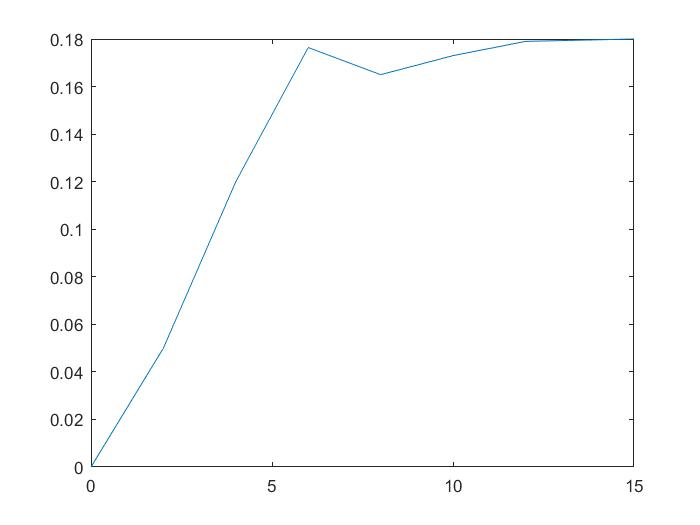
\includegraphics[height=200pt]{1.jpg}
  \item
  Distortion cure with U varying, set Y and V to 1:
  %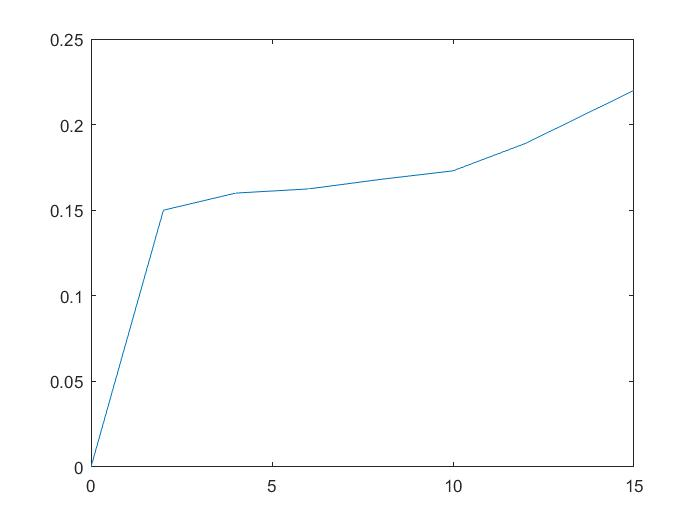
\includegraphics[height=200pt]{2.jpg}
  \item
  Distortion cure with V varying, set U and Y to 1:
  %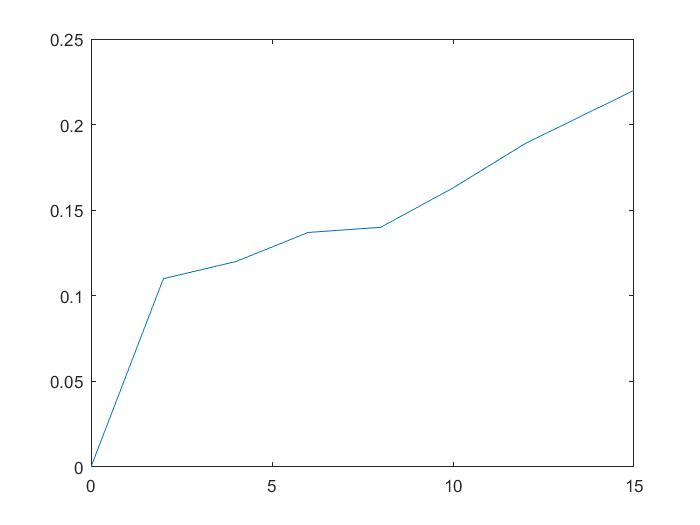
\includegraphics[height=200pt]{3.jpg}
\end{itemize}
	The pattern is that the error rate increases fast, then slow down up to a limit.\\
	First, the average error rates for these three settings are increasing with the sub-sampling factor increasing. Another observation is that Y value is much important compared to the other two values since the error rate increases much faster.\\
  \section*{Q 2}
     The main idea is to subsample differently. For example, instead of sampling with a constant sample interval, for particular image, the histogram is different and the distribution of the texture is  way more different. So, with some calculations like gradient, smaller sample interval is applied to complex part of the image.\\
     Another easier way is to increase the total bits for the image.\\
     Some output results are as followed:\\
     %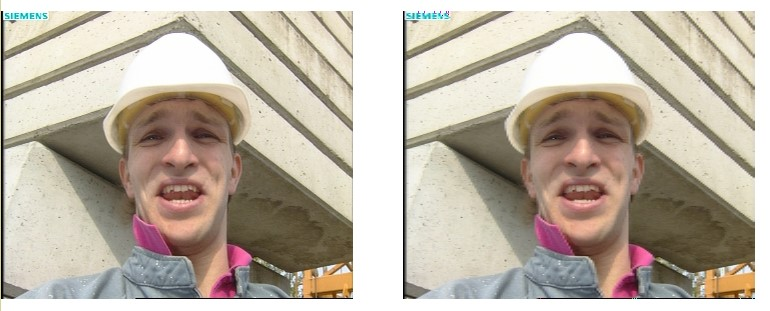
\includegraphics[height=150pt]{4.jpg}
     optimized one with Y=4\\
      %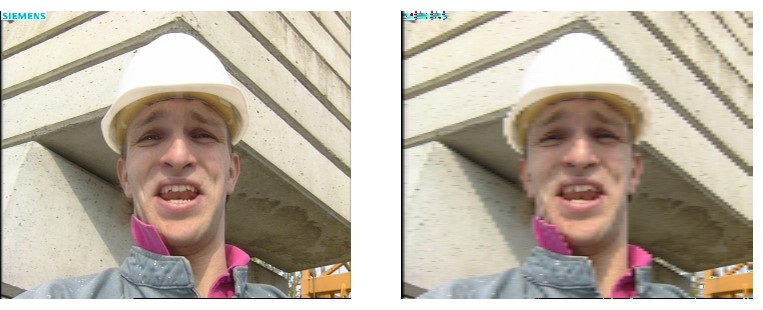
\includegraphics[height=150pt]{5.jpg}
      original image with Y=4.
     
\end{document}                          % The required last line
